For determining and controlling the attitude of the spacecraft, a brief study should be done to examine any disturbance in the space environment that may generate extra torque to change the position and orientation of the spacecraft.

A satellite's attitude is influenced by a myriad of different disturbances. These can include both internal disturbances caused by the satellite and external disturbances. Because the disturbances affect the satellite as torques, they are also referred to as torques in this section. 

Aerodynamic drag in the upper earth's atmosphere, the magnetic and gravitational field, solar radiation pressure, and pressure from micrometeorites impacts are the primary external disturbances. However, in orbits around the Earth, the last mentioned is unlikely to take place \cite{wertz2012spacecraft}. Moreover, the solar radiation induced torque has low order of magnitude when compared with the aforementioned perturbations. These dominant regions are influenced by the geometry and mass distribution of the satellite in question. The external disturbances relevant to cubesat are described in detail in the following sections and are based on \cite{wertz2012spacecraft, wie1998space}.

The total external disturbance torque in the BRF is given by
\begin{equation}
    \mathbf{M}_{\text{ext.}} = \mathbf{M}_{\text{drag}} + \mathbf{M}_{\text{GG}} + \mathbf{M}_{\text{mrs.}} 
\end{equation}


\section{Gravity Gradient Disturbance}
The components of the gravity vector change along the orbit of the satellite due to its non-symmetric nature and finite dimensions. The variation in the gravity components results in a gravitational torque applied on the body which makes a rotational effect on the body.

The gravitational force element $d\mathbf{F}_i$ acting on mass element $dm_i$ has a position vector $\mathbf{R}_i$ relative to the geocenter is defined as
\begin{equation}
    d\mathbf{F}_i = -\frac{\mu \mathbf{R}_i}{R_i} dm_i; \quad \mu \triangleq GM_{\oplus} 
\end{equation}
The torque induced from this element force $d\mathbf{F}_i$ about the spacecraft's geometric center, at position $\mathbf{r}_i$ relative to spacecraft's geometric center can be expressed as
\begin{equation}
    d\mathbf{N}_i = \mathbf{r}_i \times d\mathbf{F}_i = (\boldsymbol{\rho} + \mathbf{r^{\prime}}) \times d\mathbf{F}_i
\end{equation}
as shown in figure \ref{fig:GG}.
\begin{figure}[H]
    \centering
    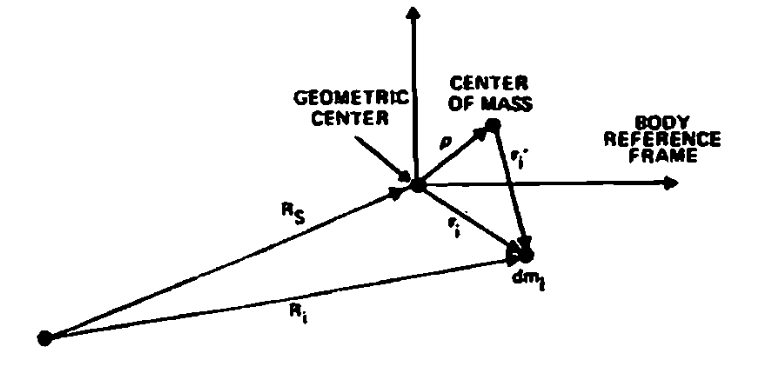
\includegraphics[width = 0.7\textwidth]{Figures/grav_grad.png}
    \caption{Coordinate System for the Calculation of Gravity-Gradient Torque}
    \label{fig:GG}
\end{figure}
The total gravity-gradient torque acting on the entire spacecraft is then given by equation
\begin{equation}
\mathbf{M}_{G G}=\int \mathbf{r}_{i} \times \mathrm{d} \mathbf{F}_{i}=\int\left(\boldsymbol{\rho}+\mathbf{r}_{i}^{\prime}\right) \times \frac{-\mu \mathbf{R}_{i}}{R_{i}^{3}} \mathrm{~d} m_{i}
\end{equation}

The geocentric position vector for the \textit{i}th mass element can be expressed in terms of the geocentric position vector of the origin of the body reference frame, $\mathbf{R}_s$, as
\begin{equation}
    \mathbf{R}_i = \mathbf{R}_s + \mathbf{r}_i = \mathbf{R}_s + \boldsymbol{\rho}+\mathbf{r^{\prime}}_i
\end{equation}
For a real satellite situation $\mathbf{R}_{i}=\mathbf{R}_{S}+\boldsymbol{\rho}+\mathbf{r}_{i}^{\prime} \gg \boldsymbol{\rho}+\mathbf{r}_{i}^{\prime}$, then
\begin{equation}
\mathbf{R}_{i}^{-3} \approx \mathbf{R}_{s}^{-3}\left[1-\frac{3 \boldsymbol{R}_{s}\left(\boldsymbol{\rho}+\boldsymbol{r}_{i}^{\prime}\right)}{R_{s}^{2}}\right]    
\end{equation}
The gravity gradient can be written as
\begin{equation} \label{eqn:GG}
    \mathbf{M}_{G G}=\frac{\mu M}{R_{S}^{2}}\left(\boldsymbol{R}_{s} \times \boldsymbol{\rho}\right)+\frac{3 \mu}{R_{s}^{3}} \int\left(\mathbf{r}{}_{i} \times {\boldsymbol{R}_s}\right)\left(\mathbf{r}_{i} \cdot {\boldsymbol{R}_{{s}}}\right) d m_{i}
\end{equation}
According to \cite{wertz2012spacecraft} equation \ref{eqn:GG} can be simplified as
\begin{equation}
\mathbf{M}_{G G}=\dfrac{3 \mu}{R_{s}^{3}}\left( \mathbf{R}_s \times([\mathbf{I}] \cdot \mathbf{R_{s}}) \right)
\end{equation}

\section{Aerodynamic Disturbance}
Aerodynamic drag is caused by atmospheric molecules colliding with the satellite's surface. For spacecraft orbiting below approximately 400 km, the aerodynamic torque disturbance is the dominant one \cite{wertz2012spacecraft}.

The force, $d\mathbf{F}_{\text{drag}}$, on a surface element $dA$, with outward normal $\hat{\mathbf{N}}$, is given by
\begin{equation}\label{eqn:Td}
d \mathbf{F}_{\text{drag}}=-\frac{1}{2} C_{D} \rho \left\|\mathbf{V}_{s a t}\right\|^{2}\left(\hat{\mathbf{N}} \cdot \hat{\mathbf{V}}_{s a t}\right) \hat{\mathbf{V}}_{s a t} d A
\end{equation}
The drag coefficient $C_D$ is usually lay between 1 and 2. A value of 2 is a good estimate for $C_D$, in cases where the aerodynamic coefficient is undetermined. 

It is important to consider that the atmospheric density is not constant with altitude. Vallado \cite{vallado2001fundamentals} presented an exponential model for density which is valid for the altitudes varying from 0 to 1000 Km. 
\begin{equation}
\rho=\rho_{o} \operatorname{EXP}\left[-\frac{h_{e l l p}-h_{o}}{H}\right]
\end{equation}
Where the data concerning this equation is given in \cite{vallado2001fundamentals}.

\noindent Equation \ref{eqn:Td} becomes
\begin{equation}
\mathbf{F}_{\text{drag}}=-\frac{1}{2} C_{D} \rho \left\|\mathbf{V}_{s a t}\right\|^{2}\left(\hat{\mathbf{N}} \cdot \hat{\mathbf{V}}_{s a t}\right) \hat{\mathbf{V}}_{s a t} A
\end{equation}
and the total aerodynamic disturbance is found to be
\begin{equation}
    \mathbf{M}_{\text{drag}} = \sum \mathbf{R} \times \mathbf{F}_{\text{drag}}
\end{equation}

\section{Magnetic Field Residual Disturbance}
residual magnetic torque $\mathbf{M}_{\text{mrs}}$ is caused by the interaction of the satellite's magnetic moment and the geomagnetic field, which is given as \cite{hughes2012spacecraft}
\begin{equation}
    \mathbf{M}_{\text{mrs}} = \mathbf{m} \times \mathbf{B}
\end{equation}
where:\\
$\mathbf{m}$ is the effective magnetic dipole moment of the satellite. \\
$\mathbf{B}$ is the Earth’s magnetic field. \\
\noindent For the case here $\mathbf{m} = \begin{bmatrix}
0.001 & 0.001 & 0.001
\end{bmatrix} \mathrm{~Am^2}$
\clearpage